
% \documentclass{article}

% % Language setting
% % Replace `english' with e.g. `spanish' to change the document language
% \usepackage[english]{babel}

% % Set page size and margins
% % Replace `letterpaper' with `a4paper' for UK/EU standard size
% \usepackage[letterpaper,top=2cm,bottom=2cm,left=3cm,right=3cm,marginparwidth=1.75cm]{geometry}

% % Useful packages
% \usepackage{amsmath}
% \usepackage{graphicx}
% \usepackage[colorlinks=true, allcolors=blue]{hyperref}


\documentclass[11pt]{article}
\usepackage[hmargin=1in,vmargin=1in]{geometry}
\usepackage{xcolor}
\usepackage{amsmath,amssymb,amsfonts,url,sectsty,framed,tcolorbox,framed}
\newcommand{\pf}{{\bf Proof: }}
\newtheorem{theorem}{Theorem}
\newtheorem{lemma}{Lemma}
\newtheorem{proposition}{Proposition}
\newtheorem{definition}{Definition}
\newtheorem{remark}{Remark}
\newcommand{\qed}{\hfill \rule{2mm}{2mm}}


\begin{document}
%%%%%%%%%%%%%%%%%%%%%%%%%%%%%%%%%%%%%%%%%%%%%%%%%%%%%%%%%%%%%%%%%%%%%
\noindent
\rule{\textwidth}{1pt}
\begin{center}
{\bf [CS304] Introduction to Cryptography and Network Security}
\end{center}
Course Instructor: Dr. Dibyendu Roy \hfill Winter 2023-2024\\
Scribed by: Raghav Agiwal (202151124) \hfill Lecture (Week 2\))
\\
\rule{\textwidth}{1pt}
%%%%%%%%%%%%%%%%%%%%%%%%%%%%%%%%%%%%%%%%%%%%%%%%%%%%%%%%%%%
%write here

\section{Hill Cipher}

\begin{itemize}
    
Hill cipher is an encryption algorithm used in cryptography. It operates on blocks (groups of letters) of plaintext and converts them into ciphertext using a matrix technique. The main idea is to perform a mathematical operation on the text using a matrix as the encryption key.\\
The Hill cipher is a substitution cipher in which each letter in the text is replaced with the corresponding number and a matrix is used to check the resulting number.\\\
The Hill cipher is an important algorithm in which the message is divided into blocks of the same size, usually a pair of letters. Each block is then treated as a vector and divided by the
matrix (key encryption matrix) to create the encrypted block. The resulting block of ciphertext can be decrypted using the inverse of the encryption key matrix.
Here we use the key K expression as matrix.\\\\

\[ K = \begin{bmatrix} a_{11} & a_{12} & \cdots & a_{1n} \\ a_{21} & a_{22} & \cdots & a_{2n} \\ \vdots & \vdots & \ddots & \vdots \\ a_{n1} & a_{n2} & \cdots & a_{nn} \end{bmatrix} \]

Assuming that our plaintext is M and our ciphertext is C, we can do the encryption and decryption process as follows:\\\\
Encryption : \[ C = M \cdot K \, (\bmod \, 26) \]
Decryption :  \[ M = C \cdot K^{-1} \, (\bmod \, 26) \]
\\\\
In these formulas C represents the ciphertext matrix, M represents the plaintext matrix, and K is the key matrix. The mod 26 denotes the modulo operation to keep the values within the range of the alphabet (A-Z).
\\\\
Let's use the word "RAGHAV" as the plaintext and encrypt it using the Hill Cipher with a 2x2 matrix key. We'll choose a key matrix for illustration:\\\\
\\
\textbf{Encryption Example:}\\
\\
\textbf{Key Matrix:}
\\
\[ K = \begin{bmatrix} 2 & 3 \\ 1 & 4 \end{bmatrix} \]

\textbf{Plaintext:}
\\
\[ P = \begin{bmatrix} 17 \\ 0 \\ 6 \\ 7 \\ 0 \\ 21 \end{bmatrix} \]  (Numerical equivalent of 'R', 'A', 'G', 'H', 'A', 'V')\\
\\
\textbf{Encrypted Matrix:}
\\
\[ C = K \cdot P \, \text{mod} \, 26 \]
\[ C = \begin{bmatrix} 11 \\ 17 \\ 21 \\ 1 \\ 17 \\ 17 \end{bmatrix} \]
\\
\textbf{Ciphertext:}\\
\\
Converting the numerical values back to letters:\\
\\
\[ \text{Ciphertext} = \text{KQUMRA} \]

So, if we encrypt the plaintext 'RAGHAV' using the key matrix K, we get the ciphertext "KQUMRA" using the hill cipher.\\

 \subsection{Symmatric key types}
\\
\subsubsection{Block Cipher}A block cipher is a basic cipher that works based on the size of a file, encrypting or decrypting each block independently. In case of symmetric key encryption, block ciphering uses the same key for encryption and decryption. The Hill cipher is essentially a symmetric block cipher, although it operates on matrices rather than large blocks.
\\\\
\subsubsection{Stream Cipher}Work on each digit (bit or group of bytes) of the plaintext simultaneously to create a ciphertext stream. Stream ciphers are often used to encrypt data continuously, bit by bit, or byte by byte, and often include pseudo-random key stream generators. The keystream is combined with the plaintext using a bitwise XOR function to produce the ciphertext stream.
\\\\

    \item \subsection{Block Cipher in detail:}
    \subsubsection{Key components of Block cipher:}
    
 \item \textbf{Plaintext:} The original data to be encrypted.\\
        \item \textbf{Ciphertext:} The encrypted result produced by the block cipher.\\
        \item \textbf{Key:} A secret key shared between the sender and receiver for encryption and decryption.\\
        \item \textbf{Block Size:} The fixed-size blocks into which the plaintext is divided.\\
        \item \textbf{Substitution-Permutation Network (SPN):} Core structure of many block ciphers, consisting of substitution (S-boxes) and permutation (P-boxes) operations\\\\

    \textbf{Example}
Let's assume our block size is 3 bits. Our sacred letter is "101" and its key is "110". We will use transformation and permutation operations in a simple way.\\

Plaintext: 101\\
Key: 110\\\\

 \subsection{Substitution-Permutation Network (SPN)}

 \subsubsection{Substitution (S-box):} Replace each block of plaintext with a corresponding value from the S-box.\\

Substitute: 101 -> 011\\

 \subsubsection{Permutation (P-box):}  Permute the bits of the substituted block.

Permute: 011 -> 101\\

\subsubsection{Key Mixing (XOR with Key):}
XOR the permuted block with the key.
\\
XOR with Key: 101 XOR 110 -> 011
\\
\textbf{Final Result:}
Ciphertext: 011\\
The final result '011' is the ciphertext corresponding to the plaintext '101' using the key '110' and the specified S-box and P-box operations.


\begin{figure}
    \centering
    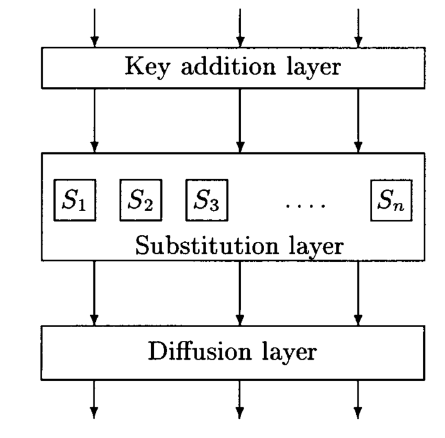
\includegraphics[width=0.4\textwidth]{image2.1.PNG} % Replace "your_image_filename" with the actual filename of your image
    \caption{} % Leave the caption empty if you don't want a label
\end{figure}

\end{itemize}

\subsection{Feistel Network}
Feistel networks have many functions where data is split into two parts. Each round applies an operation to one half of the data and uses the result to replace the other half. Then swap the halves and repeat the process for more matches. The final result is the ciphertext.
\\

\subsection*{Formula:}
Let's denote the plaintext as $L_0R_0$, where $L_0$ is the left half and $R_0$ is the right half. After each round $i$, the Feistel function $F$ is applied to the right half, and the result is used to modify the left half. The halves are then swapped.

The Feistel Network structure can be represented as:

\[
\begin{align*}
L_{i+1} &= R_i \\
R_{i+1} &= L_i \oplus F(R_i, K_i)
\end{align*}
\]

where:
\begin{itemize}
    \item $L_{i+1}$ and $R_{i+1}$ are the left and right halves after round $i+1$.
    \item $R_i$ and $L_i$ are the right and left halves after round $i$.
    \item $F$ is the Feistel function.
    \item $K_i$ is the round key for round $i$.
    \item $\oplus$ denotes the bitwise XOR operation.
\end{itemize}

\subsection*{Encryption:}
\textbf{Initialization:} Split the plaintext into left and right halves ($L_0$ and $R_0$).

\textbf{Rounds:} For each round $i$:
\begin{align*}
L_{i+1} &= R_i \\
R_{i+1} &= L_i \oplus F(R_i, K_i)
\end{align*}

\textbf{Final Swap:} Swap $L_{\text{final}}$ and $R_{\text{final}}$ to get the final ciphertext.

\subsection*{Decryption:}
The decryption process is the same as encryption, but the round keys are used in reverse order. The process is as follows:

\textbf{Initialization:} Split the ciphertext into left and right halves ($L_{\text{final}}$ and $R_{\text{final}}$).

\textbf{Rounds (in reverse order):} For each round $i$:
\begin{align*}
R_i &= L_{i+1} \\
L_i &= R_{i+1} \oplus F(L_{i+1}, K_i)
\end{align*}

\textbf{Final Swap:} Combine $L_0$ and $R_0$ to get the final decrypted plaintext.


\begin{figure}
    \centering
    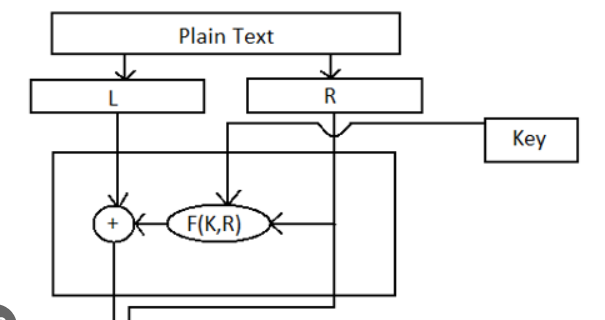
\includegraphics[width=0.6\textwidth]{image2.2.PNG} % Replace "your_image_filename" with the actual filename of your image
    \caption{} % Leave the caption empty if you don't want a label
\end{figure}



\subsection{Iterated Block Cipher:}
Iterative block cipher is an important encryption algorithm that uses the block cipher multiple times in sequence (iterations) to increase security. Repeated application of the block cipher helps achieve higher levels of obfuscation and propagation, making it resistant to various cryptographic attacks.
\\
There are many variations of a block cipher; each variation usually involves repetition of certain operations such as substitutions, substitutions, and key combinations.\\

\subsection*{Formula:}
Let's denote the plaintext as $P$, and the iterated block cipher process can be represented as:
\[ C = E_K^n(P) \]
where:
\begin{itemize}
    \item $C$ is the ciphertext.
    \item $E_K^n$ represents the application of the block cipher with key $K$ for $n$ rounds.
    \item $P$ is the plaintext.
\end{itemize}

\subsection*{Encryption:}
The encryption process involves applying the block cipher multiple times to the plaintext:
\[ C = E_K^n(P) \]

\subsection*{Decryption:}
The decryption process is the reverse of encryption, applying the block cipher in the reverse direction (using the inverse operations or the decryption algorithm) for the same number of rounds:
\[ P = D_K^n(C) \]
where:
\begin{itemize}
    \item $D_K^n$ represents the decryption of the block cipher with key $K$ for $n$ rounds.
\end{itemize}

\subsection*{Example:}
Let's consider a simplified iterated block cipher with three rounds, denoted as $E_K^3$. The encryption process would involve applying the block cipher three times:
\[ C = E_K^3(P) = E_K(E_K(E_K(P))) \]
And the decryption process would involve applying the block cipher in the reverse direction for three rounds:
\[ P = D_K^3(C) = D_K(D_K(D_K(C))) \]

It's important to note that in practical applications, the number of rounds, the choice of block cipher, and the key schedule are crucial factors in determining the security of the iterated block cipher. Common examples of iterated block ciphers include the Advanced Encryption Standard (AES) and the Data Encryption Standard (DES).

\\\\

\section*{Data Encryption Standard (DES)}

\subsection*{Definition:}
The Data Encryption Standard (DES) is a symmetric-key block cipher that was widely used as a standard for secure communication and data protection. Developed by IBM and adopted as a federal standard in the United States in the 1970s, DES was later replaced by the Advanced Encryption Standard (AES) due to concerns about its key size.

\subsection*{Encryption Process:}
\textbf{Initial Permutation (IP):}
\[ IP(PT) \]

\textbf{Key Schedule:}
The 64-bit key is expanded and used to generate 16 subkeys, one for each round.

\textbf{Rounds (16 rounds):}
Each round consists of:
\begin{itemize}
    \item \textbf{Expansion:} Expanding the 32-bit right half to 48 bits.
    \item \textbf{Substitution:} Substituting using S-boxes.
    \item \textbf{Permutation:} Permuting the 32-bit result.
    \item \textbf{XOR with Left Half:} XOR the result with the left half of the data.
\end{itemize}
The process is repeated for 16 rounds.

\textbf{Final Permutation (FP):}
\[ FP(R_{16}L_{16}) \]

\subsection*{Decryption Process:}
The decryption process is the reverse of encryption. The ciphertext undergoes the same processes, but the subkeys are used in reverse order.

\textbf{Initial Permutation (IP):}
\[ IP(C) \]

\textbf{Key Schedule:}
The same key schedule generates subkeys in reverse order.

\textbf{Rounds (16 rounds):}
Each round's processes are applied in reverse order.

\textbf{Final Permutation (FP):}
\[ FP(R_{16}L_{16}) \]

\subsection*{Key Generation (Key Schedule):}
\textbf{Permutation Choice 1 (PC-1):}
\[ PC-1(Key) \]

\textbf{Key Splitting:}
The 56-bit key is split into two 28-bit halves.

\textbf{Round Key Generation (Shifts and Permutations):}
\[ K_i = PC-2(Shift(PC-1(Key))) \]


\begin{figure}
    \centering
    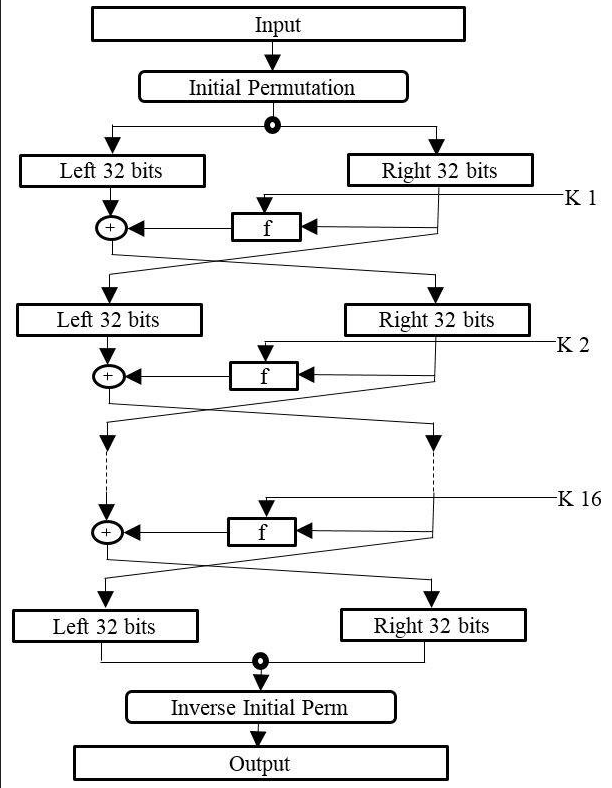
\includegraphics[width=0.4\textwidth]{image2.3.PNG} % Replace "your_image_filename" with the actual filename of your image
    \caption{} % Leave the caption empty if you don't want a label
\end{figure}



\subsection*{Formulas:}
\textbf{Initial Permutation (IP):}
\[ IP(PT) \]

\textbf{Final Permutation (FP):}
\[ FP(R_{16}L_{16}) \]

\textbf{Round Encryption (Example for Round i):}
\[ R_{i+1} = L_i \oplus f(R_i, K_i) \]
\[ L_{i+1} = R_i \]

where:
\begin{itemize}
    \item \(L_i\) and \(R_i\) are the left and right halves of the data at round \(i\).
    \item \(K_i\) is the subkey for round \(i\).
    \item \(f\) is the round function combining expansion, substitution, permutation, and XOR operations.
\end{itemize}

\textbf{Round Key Generation:}
\[ K_i = PC-2(Shift(PC-1(Key))) \]

DES is considered insecure by today's standards due to its small key size. For secure communication, it has been largely replaced by more advanced encryption algorithms like AES.


\end{document}


